\documentclass[../book.tex]{subfiles}

\chapter{Introduction: Into the Data}
\label{ch:introduction}

\begin{quote}
\emph{Definition}: A computer program is said to \textbf{learn} from
experience \(E\) with respect to some class of tasks \(T\) and
performance measure \(P\), if its performance at tasks in \(T\),
improves with experience \(E\) \autocite[2]{Mitchell_1997}.
\index{Mitchell, Tom} \index{machine learner!computer program as}
\end{quote}

\begin{quote}
In the past fifteen years, the growth in algorithmic modeling
applications and methodology has been rapid. It has occurred largely
outside statistics in a new community---often called machine
learning---that is mostly young computer scientists. The advances,
particularly over the last five years, have been startling
\autocite[200]{Breiman_2001} \index{Breiman, Leo}
\end{quote}

\begin{quote}
The key question isn't `How much will be automated?' It's how we'll
conceive of whatever \emph{can't} be automated at a given time.
\autocite[77]{Lanier_2013}
\end{quote}

A relatively new field of scientific-engineering devices said to `learn
from experience' \index{learning!from experience} has become operational
in the last three decades. Known by various names -- machine learning,
pattern recognition, knowledge discovery, data mining -- the field and
its devices, which all take shape as computer programs or code,
\index{code!machine learning as} seem to have quickly spread across
scientific disciplines, business and commercial settings, industry,
engineering, media, entertainment and government. Heavily dependent on
computation, they are found in breast cancer research, in autonomous
vehicles, in insurance risk modelling, in credit transaction processing,
in computer gaming, in face and handwriting recognition systems, in
astronomy, advanced prosthetics, ornithology, finance, surveillance (see
the U.S. Government's \texttt{SkyNet} for one example of a machine
learning surveillance system \autocite{NationalSecurityAgency_2012}) or
robots( see a Google robotic arm farm learning to sort drawers of office
equipment such as staplers, pens, erasers and paper clips
\autocite{Levine_2016}. \index{machine learner!Skynet}

Sometimes machine learning devices are understood as \emph{scientific
models}, and sometimes they are understood as \emph{operational
algorithms}. In very many scientific fields, publications mention or
describe these techniques as part of their analysis of some experimental
or observational data (as in the logistic regression classification
models found in many biomedical papers).
\index{machine learner!logistic regression} They anchor the field of
`data science' \autocite{Schutt_2013}, as institutionalised in several
hundred data science institutes scattered worldwide.
\index{data science!relation to machine learning} Not so recently, they
also became mundane mechanisms deeply embedded in other systems or
gadgets (as in the decision tree models used in some computer game
consoles to recognise gestures, the neural networks used to recognise
voice commands by search engine services such as \texttt{Google\ Search}
\index{Google Search} and \texttt{Apple\ Siri} \index{Apple Siri}
\autocite{McMillan_2013} or Google's \texttt{TensorFlow} software
packages that puts deep convolutional neural nets on Android devices
\autocite{Google_2015a}\index{Google!TensorFlow}). In platform settings,
they operate behind the scenes as part of the everyday functioning of
services ranging from player ranking in online games to border control
face recognition, from credit scores to news feeds on Facebook
\index{Facebook!news feed}.

In all of these settings, applications and fields, machine learning is
said to transform the nature of knowledge. Might it transform the
practice of critical thought? This book is an experiment in such
practice. \index{critical thought!practice of}

\section{Three accumulations: settings, data and
devices}\label{three-accumulations-settings-data-and-devices}

Three different accumulations cross-stratify in machine learning:
settings, data and devices. The volume and geography of searches on
Google Search provides some evidence of the diverse settings or sites
doing machine learning. If we search for terms such as
\texttt{artificial\ intelligence,\ machine\ learning} and
\texttt{data\ mining} on the \href{http://www.google.com/trends}{Google
Trends} service \index{Google!Google Trends}, the results for the last
decade or so suggest shifting interest in these topics.

\begin{figure}
  \centering
      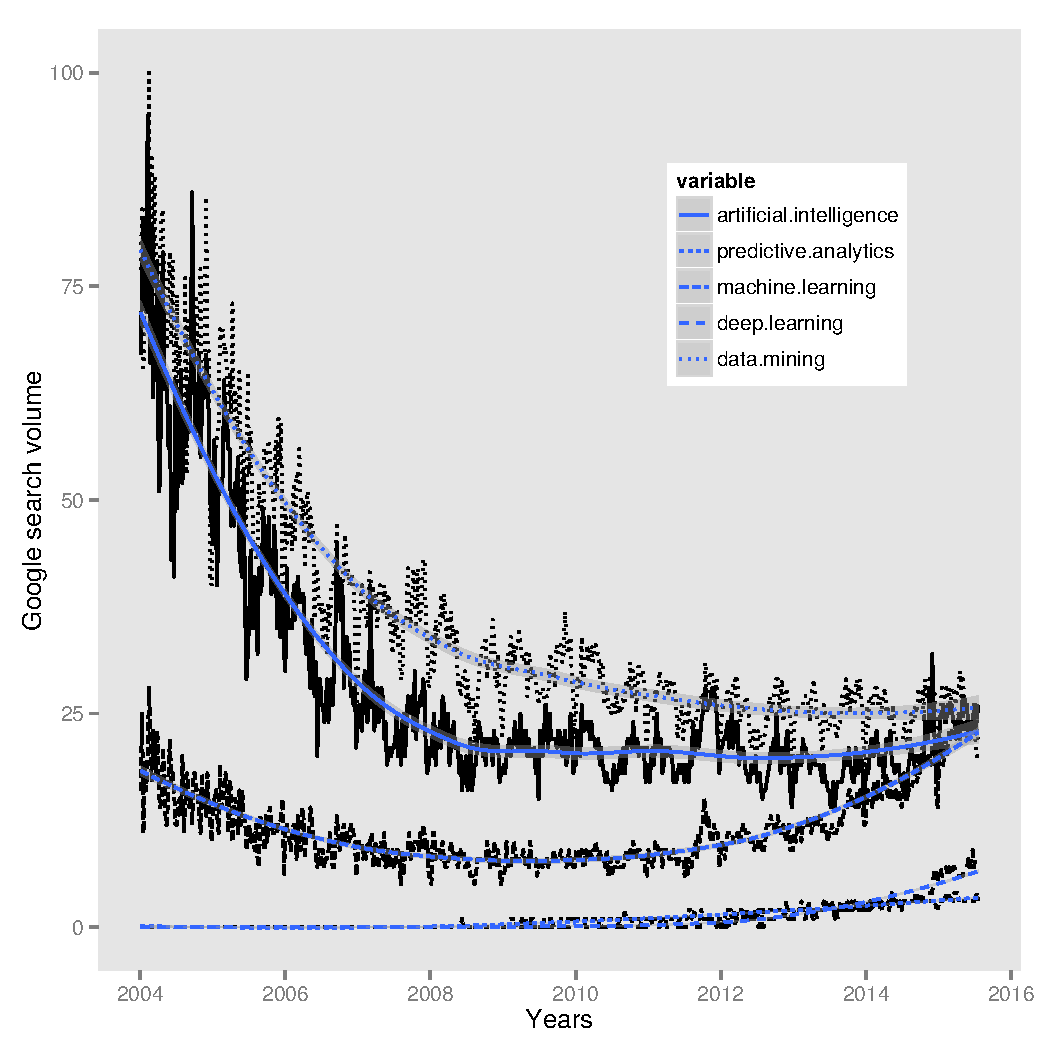
\includegraphics[width=0.9\textwidth]{figure/google_trends-1.pdf}
        \caption[Google Trends search volume for machine learning]{Google Trends search volume for `machine learning` and related query terms in English, globally 2004-2016}
  \label{fig:google_trends}
\end{figure}

In Figure \ref{fig:google_trends}, two general search terms that had a
very high search volume in 2004 -- `artificial intelligence' and `data
mining' \index{artificial intelligence} \index{data mining} -- slowly
decline over the years before starting to increase again in the last few
years. By contrast, \texttt{machine\ learning} loses volume until around
2008, and then gradually rises again so that by mid-2016 it exceeds the
long-standing interests in data-mining and artificial intelligence.
Whatever the difficulties in understanding GoogleTrends results, these
curves suggest an accumulation of sites and settings turning towards
machine learning.\footnote{In the plot (Figure \ref{fig:google_trends},
  the weekly variations in search volume on Google give rise to many
  spikes in the data. These spikes can be linked to specific events such
  as significant press releases, public debates, media attention and
  film releases. It is hard to know who is doing these searches. The
  data provided by Google Trends includes geography, and it would be
  interesting to compare the geographies of interest in the different
  terms over time.} \index{accumulation!of settings} What does it mean
that machine learning surfaces in so many different places, from fMRIs
to Facebook's \texttt{AI-Flow} \autocite{Facebook_2016},
\index{Facebook!AI-Flow}, from fisheries management to Al Queda courier
network monitoring by \texttt{SkyNet}?\footnote{The diagram shown in
  Figure \ref{fig:google_trends} actually draws two lines for each
  trend. The `raw' weekly GoogleTrends data -- definitely not raw data,
  as it has been normalized to a percentage \autocite{Gitelman_2013} --
  appears in the very spiky lines, but a much smoother line shows the
  general trend. This smoothing line is the work of a statistical model
  -- a local regression or loess model \autocite{Cleveland_1992}
  \index{Cleveland, William} developed in the late 1970s.
  \index{statistics!model!local regression} The line depends on
  intensive computation and models (linear regression, \emph{k} nearest
  neighbours, \index{machine learner!k-nearest neighbors}
  \index{linear regression}). The smoother lines make the spiky weekly
  search counts supplied by Google much easier to see. They construct
  alignments in the data by replacing the irregular variations with a
  curve that unequivocally runs through time with greater regularity.
  The smoothed lines shade the diagram with a predictive pattern. The
  lineaments of machine learning already appear in such lines. How have
  things been arranged so that smooth lines run through an accumulated
  archive of search data?} \index{machine learner!Skynet}

\begin{figure}
  \centering
      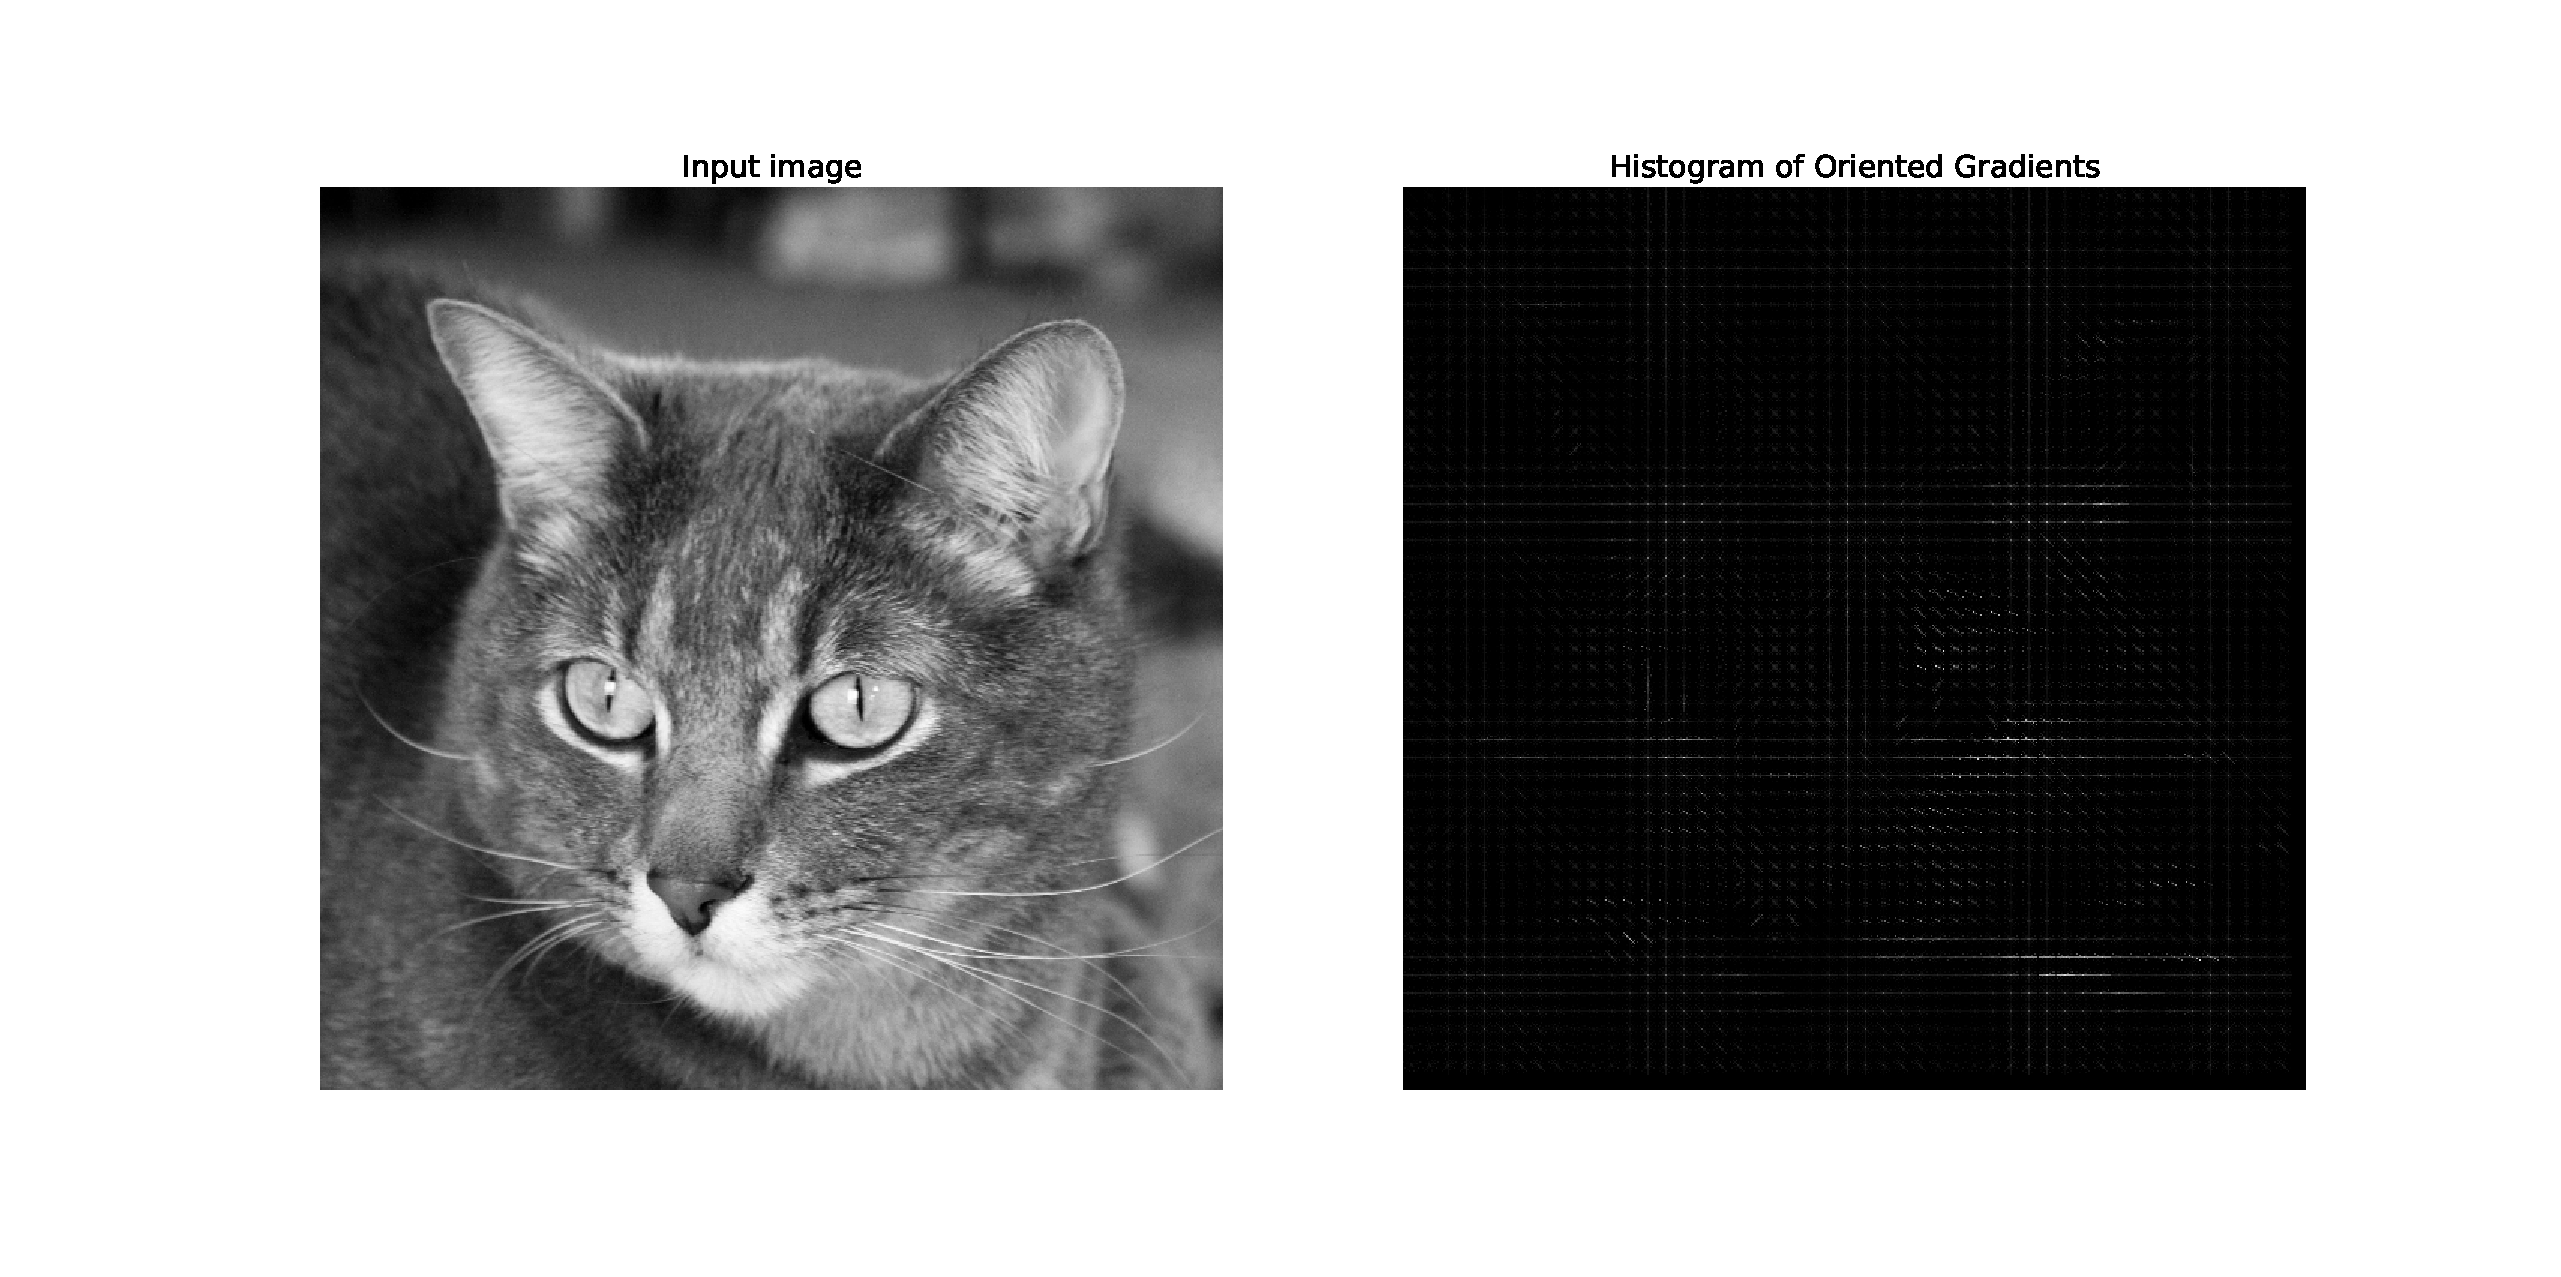
\includegraphics[width=0.9\textwidth]{figure/cat_hog.pdf}
        \caption[Cat as histogram of gradients]{Close up of cat. The image on the left is already signal-processed as a JPEG format file. The image on the right is further processed using histogram of oriented gradients (HOG) edge detection. \texttt{kittydar} models HOG features.  Cat photo courtesy photos-public-domain.com}
  \label{fig:cat}
\end{figure}

A second accumulation concerns the plenitude of things in the world as
data. \index{data!plenitude} If we wanted to describe the general
horizon of machine learning as a data practice in its specificity, we
might turn to cats. \index{data!practice} Cat images accumulate on
websites and social media platforms as de-centred, highly repetitive
data forms. Like the billions of search engine queries, email messages,
tweets, or much contemporary scientific data (e.g.~the DNA sequence data
discussed in chapter \ref{ch:genome}), images accumulate in archives of
communication.\index{image recognition} Take the case of
\texttt{kittydar,} a machine learner in the area of image recognition
(see \href{http://harthur.github.io/kittydar}{kittydar}): `Kittydar is
short for kitty radar. Kittydar takes an image (canvas) and tells you
the locations of all the cats in the image' \autocite{Arthur_2012}.
\index{machine learner!kittydar} This playful piece of code demonstrates
how machine learning can be amidst mundane accumulation. Heather Arthur,
who developed \texttt{kittydar} writes: \index{Arthur, Heather}

\begin{quote}
Kittydar first chops the image up into many ``windows'' to test for the
presence of a cat head. For each window, kittydar first extracts more
tractable data from the image's data. Namely, it computes the Histogram
of Orient Gradients descriptor of the image \ldots{} This data describes
the directions of the edges in the image (where the image changes from
light to dark and vice versa) and what strength they are. This data is a
vector of numbers that is then fed into a neural network \ldots{} which
gives a number from 0 to 1 on how likely the histogram data represents a
cat. The neural network \ldots{} has been pre-trained with thousands of
photos of cat heads and their histograms, as well as thousands of
non-cats. See the repo for the node training scripts
\autocite{Arthur_2012}. \index{data!image as} \index{data!vector}
\end{quote}

This toy device finds cat heads in digital photographs, but also
exemplifies many key traits of machine learning. Large accumulations of
things become \glspl{vector} in a dataset. \index{data!vector} A dataset
is used to train a typical machine learning device, a neural net,
\index{machine learner!neural net} and the neural net \emph{classifies}
subsequent images probabilistically. The code for all this is `in the
repo.' \index{code!circulation of} Based on how it locates cats, we can
begin to imagine similar pattern recognition techniques in use in
self-driving cars \autocite{Thrun_2006}, border control facial
recognition systems, military robots or wherever something seen implies
something to do.

Faced with the immense accumulation of cat images on the internet,
\texttt{kittydar} can do very little. It only detects the presence of
cats that face forward. And it sometimes classifies people as cats. As
Arthur's description suggests, the software finds cats by cutting the
images into smaller windows. For each window, it measures a set of
gradients -- a spatial order of great significance in machine learning -
\index{gradient|see {gradient descent}} running from light and dark, and
then compares these measurements to the gradients of known cat images
(the so-called `training data')\index{data!training}. The work of
classification according to the simple categories of `cat' or `not cat'
\index{classification} is given either to a neural network (as discussed
in chapter \ref{ch:subjects}, a typical machine learning technique and
one that has recently been heavily developed by researchers at Google
\autocite{Le_2011}, themselves working on images of cats among other
things taken from Youtube videos
\autocite{BBC_2012}\index{neural network|see {machine learner!neural net}},
or to a support vector machine (a technique first developed in the 1990s
by researchers working at IBM; see chapter \ref{ch:pattern}).
\index{support vector machine|see {machine learner!support vector machine}}

A final accumulation comprises machine learning techniques and devices.
Machine learning range from the mundane to the esoteric, from code
miniatures such as \texttt{kittydar} to the infrastructural sublime of
computational clouds and clusters twirling in internet data-streams.
Like the images that \texttt{kittydar} classifies, the names of machine
learning techniques and devices proliferate and accumulate in textbooks,
instructional courses, website tutorials, software libraries and code
listings: linear regression\index{linear regression}, logistic
regression, \index{machine learner!logistic regression} neural
networks\index{machine learner!neural net}, linear discriminant
analysis\index{machine learner!linear discriminant analysis}, support
vector machines, \index{support vector machine} k-means clustering,
\index{machine learner!\textit{k}-means clustering} decision
trees\index{decision tree|see {machine learner!decision tree}}, \emph{k}
nearest neighbours,
\index{nearest neighbours|see {machine learner!\textit{k}-nearest neighbours}}
random forests, \index{principal component analysis} principal component
analysis, or naive Bayes \gls{classifier}
\index{machine learner!Naive Bayes} to name just some of the most
commonly used. Sometimes they have proper names: \texttt{RF-ACE},
\texttt{Le-Net5}, or \texttt{C4.5}. These names refer to predictive
models and to computational algorithms of various ilk and provenance.
Intricate data practices -- normalization, regularization,
cross-validation, feature engineering, feature selection, optimisation
\index{data!practice} -- embroider datasets into shapes they can
recognise. The techniques, algorithms and models are not necessarily
startling new or novel. They take shape against a background of more
than a century of work in mathematics, statistics, computer science as
well as disparate scientific fields ranging from anthropology to
zoology. Mathematical constructs drawn from linear algebra, differential
calculus, numerical optimization and probability theory pervade practice
in the field. \index{mathematics} Machine learning itself is an
accumulation rather than a radical transformation.

\section{Who or what is a machine
learner?}\label{who-or-what-is-a-machine-learner}

I am focusing on machine learners \index{machine learner|textbf} -- a
term that refers to both humans and machines or human-machine relations
\index{human-machine relations} throughout this book -- situated amidst
these three accumulations of settings, data and devices. While it is not
always possible to disentangle machine learners from the databases,
infrastructures, platforms or interfaces they work through, I will argue
that data practices associated with machine learning delimit a
\textit{\gls{positivity}} of knowing. \index{positivity!of knowledge}
The term `positivity' comes from Michel Foucault's \emph{The Archaeology
of Knowledge} \autocite{Foucault_1972}, and refers to specific forms of
accumulation of \glspl{statement} grouped in a discursive practice.
Analyzed archaeologically, a positivity can be investigated and
inhabited to some degree by critical thought.

Foucault attributes a lift-off effect to positivity:

\begin{quote}
The moment at which a discursive practice achieves individuality and
autonomy, the moment therefore at which a single system for the
formation of statements is put into operation, or the moment at which
this system is transformed, might be called the threshold of positivity.
\autocite[186]{Foucault_1972}\index{positivity!threshold of}\index{Foucault, Michel!positivity}
\end{quote}

Machine learners today circulate into domains that lie far afield of the
eugenic and psychology laboratories, industrial research institutes or
specialized engineering settings in which they first took shape (in some
cases, such as the linear regression model or principal component
analysis, more than a century ago; in others such as support vector
machines or random forests, in the last two decades). If they are not
exactly new and have diverse genealogies, the question is: what happen
as machine learners shift from localized mathematical or engineering
techniques to an everyday device that can be generalized to locate cats
in digital images, the Higgs boson in particle physics experiments or
fraudulent credit card transactions? Does the somewhat unruly
generalization of machine learning \index{generalization} across
different epistemic, economic, institutional settings -- the pronounced
uptick shown in Figure \ref{fig:google_trends} -- attest to a
re-definition of knowledge, decision and control, a new
\gls{operational formation} \index{operational formation} in which `a
system is transformed'?

\section{Algorithmic control to the machine
learners?}\label{algorithmic-control-to-the-machine-learners}

Written in code, machine learners operate as programs or computational
processes to produce statements that may take the form of numbers,
graphs, propositions (see for instance the propositions produced by a
recurrent neural net on the text of this book in the concluding chapter
\ref{ch:conclusion}).\index{statements!forms of} Machine learning can
also be viewed as a change in how programs or the code that controls
computer operations are developed and operate (see chapter
\ref{ch:diagram} for more detailed discussion of this).
\index{code!writing of} The term `learning' in machine learning points
to this change and many machine learners emphasize it. Pedro Domingos,
for instance, a computer scientist at the University of Washington,
writes:

\begin{quote}
Learning algorithms -- also known as learners -- are algorithms that
make other algorithms. With machine learning, computers write their own
programs, so we don't have
to.\autocite[6]{Domingos_2015a}\index{Domingos, Pedro!on machine learning}
\end{quote}

Viewed from the perspective of control, and how control is practiced,
digital computer programs stem from and epitomise the `control
revolution' \autocite{Beniger_1986} that arguably has, since the late
nineteenth century, programmatically re-configured production,
distribution, consumption, and bureaucracy by tabulating, calculating
and increasingly communicating events and
operations.\index{control!crisis of} With the growth of digital
communication networks in the form of the internet, the late 20th
century entered a new crisis of control, no longer centred on logistic
acceleration but on communication and knowledge. \index{Beniger, James}
Almost all accounts of the operational power of machine learning
emphasise its power to inflect the control of processes of communication
-- border flows, credit fraud, spam email, financial market prices,
cancer diagnosis, targeted online adverts -- processes whose unruly or
transient multiplicity otherwise evades or overwhelm us -- with
knowledge (classifications and predictions in particular) derived from
algorithms that make other algorithms. On this view, \texttt{kittydar}
can isolate cats amidst the excessive accumulation of images on the
internet because neural net learning algorithms (back-propagation,
gradient descent) have written a program -- `a pre-trained' neural net
-- during its training phase. \index{machine learner!\texttt{kittydar}}

If a newly programmatic field of knowledge-control takes shape around
machine learning, how would we distinguish it from computation more
generally? Recent critical research on algorithms offers one lead. In a
study of border control systems, which often use machine learners to do
profiling and facial recognition \index{facial recognition}, Louise
Amoore advocates attention to calculation and algorithms:

\begin{quote}
Surely this must be a primary task for critical enquiry -- to uncover
and probe the moments that come together in the making of a calculation
that will automate all future decisions. To be clear, I am not proposing
some form of humanist project of proper ethical judgement, but rather
calling for attention to be paid to the specific temporalities and norms
of algorithmic techniques that rule out, render invisible, other
potential futures \autocite{Amoore_2011}. \index{Amoore, Louise}
\end{quote}

As Amoore writes, some potential futures are being `ruled out' as
calculations automate decisions. Anna Munster \index{Munster, Anna} puts
the challenge more bluntly: `prediction takes down potential'
\autocite{Munster_2013}. I find much to agree with here. Machine
learning is a convoluted but nevertheless concrete and historically
specific form of calculation
\index{calculation|see {mathematics!calculation}} (as we will see in
exploring algebraic operations in chapter \ref{ch:vector}, in finding
and optimising certain mathematical functions in chapter
\ref{ch:function} or in characterising and shaping probability
distributions in chapter \ref{ch:probability}). It works to mediate
future-oriented decisions (although all too often, very near-future
decisions such as ad-click prediction)\index{decision}.

I am less certain about treating machine learning as automation.
Learning from data, as we will see, does often sidestep and substitute
for existing ways of acting, and practices of control, and it thereby
re-configures human-machine differences.
\index{machine learning!human-machine difference} Yet the notion of
automation does not capture well how this comes about.
\index{machine learning!as automation} The programs that machine learner
`write' are formulated as probabilistic models, as learned rules or
association, and they generate predictive and classificatory statements
(`this is a cat'). They render calculable some things which hitherto
appeared intractable to calculation (for instance, the argument of a
legal case). Such calculation, with all the investment it attracts (in
the form of professional lives, in the form of infrastructures
\index{infrastructure}, in reorganisation of institutions, corporations
and governments, etc.) does rule out some and reinforce other futures.
\footnote{As for consequences, we need only consider some of the many
  forms of work that have already been affected by or soon could be
  affected by machine learning. Postal service clerks no longer sort the
  mail because neural net-based handwriting recognition reads addresses
  on envelopes
  \index{handwriting recognition|seealso {digit recognition}}.
  Locomotives, cars and trucks are already driven by machine learners,
  and soon driving may not be same occupational cultural it was.
  Hundreds of occupational categories have to some degree or other
  machine learners in their near future. Carl Benedikt Frey and Michael
  Osborne model the chances of occupational change for 700 occupations
  using, aptly enough, the machine learning technique of Gaussian
  Processes \autocite{Frey_2013}.} If this transformed calculability is
automation, we need to understand the specific contemporary reality of
automation as it takes shape in machine learning. We cannot conduct
critical enquiry into the calculation that will automate future
decisions without opening the very notions of calculation and automation
into question.\index{calculation!historical specificity of}
\index{automation!historical specificity of}

Does the concept of algorithm help us identify the moments that come
together in machine learning without resorting to a-historical concepts
of automation or calculation? In various scholarly and political debates
around changes business, media, education, health, government or
science, quasi-omnipotent agency has been imputed to algorithms
\index{algorithm!primacy}
\autocites{Barocas_2013}{Beer_2013}{Cheney-Lippold_2011}{Fuller_2012}{Galloway_2004};
\textcite{Gillespie_2014}; \textcite{Neyland_2015};
\textcite{Pasquinelli_2014}; \textcite{Smith_2013};
\textcite{Totaro_2014}; \textcite{Wilf_2013}{]} or sometimes just `the
algorithm.' This growing body of work understands the power of
algorithms in the social science and humanities literature in different
ways, sometimes in terms of rules, sometimes as functions or
mathematical abstractions, and increasingly as a located practice. There
is general agreement that algorithms are powerful, or at least, can bear
down heavily on people's lives and conduct, re-configuring, for
instance, culture as algorithmic \autocite{Hallinan_2014}.

Some of the critical literature on algorithms identifies abstractions as
the source of their power. For instance, in his discussion of the
`metadata society,' Paolo Pasquinelli proposes that

\begin{quote}
a progressive political agenda for the present is about moving at the
same level of abstraction as the algorithm in order to make the patterns
of new social compositions and subjectivities emerge. We have to produce
new revolutionary institutions out of data and algorithms. If the
abnormal returns into politics as a mathematical object, it will have to
find its strategy of resistance and organisation, in the upcoming
century, in a mathematical way \autocite{Pasquinelli_2015}.
\index{Pasquinelli, Paolo}\index{algorithm!as abstraction}
\end{quote}

`Moving at the same level of abstraction as the algorithm' offers some
purchase as a formulation for critical practice, and for experiments in
such practice. Since in mathematics let alone critical thought,
abstraction can be understood in many different ways, any direct
identification of algorithms with abstraction will, however, be
difficult to practice. Which algorithm, what kind of abstraction and
which `mathematical way' should we focus on? Like automation and
calculation, abstraction and mathematics have mutable historicities.
\index{mathematics!historicity of} We cannot `move at the same level'
without taking that into account. Furthermore, given the accumulations
of settings, data and devices, there might not be any single level of
abstraction to move at, only a torque and flux of different moments of
abstraction at work in generalizing, classifying, circulating and
stratifying in the midst of transient and plural multiplicities.
\index{abstraction!as algorithm}

\section{The archaeology of
operations}\label{the-archaeology-of-operations}

Given mathematics and algorithms do loom large in machine learning, how
do we address their the workings without pre-emptively ascribing potency
to mathematics, or to algorithms? In the chapters that follow, I do
explore specific learning algorithms (gradient descent in chapter
\ref{ch:function} or recursive partitioning \ref{ch:pattern}) and
mathematical techniques (the sigmoid function in chapter
\ref{ch:function} or inner products in chapter \ref{ch:vector}) in
greater empirical and conceptual depth. Following much scholarship in
science and technology studies, I maintain that attention to specificity
of practices is an elementary prerequisite to understanding
human-machine relations, \index{human-machine relations!practice in} and
their transformations. The \gls{archaeology} of operations that I will
develop combines an interest in machine learning as a form of knowledge
production and a strategy of power. Like Foucault, I see no exteriority
between techniques of knowledge and strategies of power (`between
techniques of knowledge and strategies of power, there is no
exteriority, even if they have specific roles and are linked together on
the basis of their difference'
\autocite[98]{Foucault_1998}\index{knowledge!power}).
\index{archaeology!of operations}

If we understand machine learning as a data practice that re-configures
local centres of power-knowledge through a re-drawing of human-machine
relations, then the specific roles and differences associated with
machine learners in the production of knowledge should be a focus of
attention. Differences are a key concern here since many machine
learners classify things. They are often simply called
`\glspl{classifier}.' \index{classifier|see{machine learner}} Some of
the practice of difference works in terms of categories.
\texttt{Kittydar} classifies images as \texttt{cat} with some
probability, but categorisation and classification in machine learning
occurs much more widely.\footnote{John Cheney-Lippold offers a quite
  general overview of categorization work. He writes: `algorithm
  ultimately exercises control over us by harnessing these forces
  through the creation of relationships between real-world surveillance
  data and machines capable of making statistically relevant inferences
  about what that data can mean' \autocite[178]{Cheney-Lippold_2011}.
  \index{classification!algorithms for}. Much of my discussion here
  seeks to explore the space of `statistical inference of what that data
  can mean' as an operational field of knowledge production.} We might
understood the importance of categories sociologically. For instance, in
his account of media power, Nick Couldry highlights the importance of
categories and categorisation:

\begin{quote}
\emph{Category} is a key mechanism whereby certain types of ordered
(often `ritualized') practice produce power by enacting and embodying
categories that serve to mark and divide up the world in certain ways.
Without \emph{some} ordering feature of practice, such as `categories',
it is difficult to connect the multiplicity of practice to the workings
of power, whether in the media or in any other sphere. By understanding
the work of categories, we get a crucial insight into why the social
world, in spite of its massive complexity still appears to us as a
\emph{common} world \autocite[62]{Couldry_2012} \index{Couldry, Nick}
\index{categories|seealso {differences|categories}} \index{power}
\end{quote}

Orderings of categorical differences undergo a great deal of
intensification via machine learning. Categories are often simply an
existing set of classifications derived from institutionalised or
accepted knowledges (for instance, the categories of customers according
to gender or age). Machine learners also generate new categorical
workings or mechanisms of differentiation. As we will see (for instance
in chapter \ref{ch:genome} in relation to scientific data from genomes),
machine learners invent or find new sets of categories for a particular
purpose (such as cancer diagnosis or prognosis). These differentiations
may or may not bring social good. The person who finds themselves paying
a higher price for an air ticket by virtue of some unknown combination
of factors including age, credit score, home address, previous travel,
or educational qualifications experiences something of the
classificatory power.

\section{Asymmetries in common
knowledge}\label{asymmetries-in-common-knowledge}

What can critical thought, the kind of enquiry that seeks to identify
the conditions that concretely constitute what anyone can say or think
or do, learn from machine learning? If we see a massive regularization
of order occurring in machine learning, what is at stake in trying to
think through those practices? They display moments of formalisation
(especially mathematical and statistical), circulation (pedagogically
and operationally), generalization (propagating and proliferating in
many domains and settings) and stratification (the socially,
epistemically, economically and sometimes politically or ontologically
loaded re-iterative enactment of categories). I am not sure that
understanding how a support vector machine or a random forest orders
differences would change how would we relate to what we see, feel,
sense, hear or think in the face of a contemporary platform such as
Amazon's \index{Amazon!recommendations} that uses Association Rule
Mining
\index{Association Rule Mining|see{machine learner!\textit{apriori} algorithm}},
an app, a passport control system that matches faces of arriving
passengers with images in a database, a computer game, or a genetic test
(all settings in which machine learning is likely to be operating).

Machine learners themselves sometimes complain of the monolithic and
homogeneous success of machine learning. Some expert practitioners
complain of a uniformity in its applications. Jeff Hammerbacher
\index{Hammerbacher, Jeff}, previously chief research scientist at
Facebook, co-founder of a successful data analytics company called
Cloudera, and currently working also on cancer research at Mount Sinai
hospital, complained about the spread of machine learning in 2011: `the
best of my generation are thinking about how to make people click ads'
\autocite{Vance_2011} \index{advertising, online}. Leaving aside debates
about the ranking of `best minds' (a highly competitive and exhaustively
tested set of subject positions; see chapter \ref{ch:subjects}),
Hammerbacher was lamenting the flourishing use of predictive analytics
techniques in online platforms such as Twitter, Google and Facebook, and
on websites more generally, whether they be websites that sell things or
advertising space. The mathematical skills of many PhDs from MIT,
Stanford or Cambridge were wrangling data in the interests of
micro-targeted advertising. As Hammerbacher observers, they were
`thinking about how to make people click ads,' and this `thinking'
mainly took and does take the form of building predictive models that
tailored the ads shown on websites to clusters of individual preferences
and desires.

Hammerbacher's unhappiness with ad-click prediction resonates with
critical responses to the use of machine learning in the digital
humanities. \index{digital humanities!use of machine learning} Some
versions of the digital humanities make extensive use of machine
learning. To cite one example, in \emph{Macroanalysis: Digital Methods
and Literary History}, Matthew Jockers \index{Jockers, Matthew}describes
how he relates to one currently popular machine learning or statistical
modelling technique, the topic model
\index{topic model|see{machine learner!topic model}} (itself the topic
of discussion in Chapter \ref{ch:probability}; see also
\autocite{Mohr_2013}\index{Mohr, John}):

\begin{quote}
If the statistics are rather too complex to summarize here, I think it
is fair to skip the mathematics and focus on the end results. We needn't
know how long and hard Joyce sweated over \emph{Ulysses} to appreciate
his genius, and a clear understanding of the LDA machine is not required
in order to see the beauty of the result. \autocite[124]{Jockers_2013}
\index{Jockers, Matthew!on topic models}
\end{quote}

The widely used Latent Dirichlet Allocation or models provide a litmus
test of how relations to machine learning is taking shape in the digital
humanities. On the one hand, these models promise to make sense of large
accumulations of documents (scientific publications, news, literature,
online communications, etc.) in terms of underlying themes or latent
`topics.' As we will, large document collections have long attracted the
interest of machine learners (see chapter \ref{ch:probability}).
\index{data!latent variables in} On the other hand, Jockers signals the
practical difficulties of relating to machine learning when he suggests
that `it is fair to skip the mathematics' for the sake of `the beauty of
the result'. While some parts of the humanities and critical social
research exhorts closer attention to algorithms and mathematical
abstractions, other parts elides its complexity in the name of `the
beauty of the results.'

Critical thought has not always endorsed the use of machine learning in
digital humanities. \index{Galloway, Alex!on knowledge production} Alex
Galloway makes two observations about the circulation of these methods
in humanities scholarship. The first points to its marginal status in
increasingly machine-learned media cultures:

\begin{quote}
When using quantitative methodologies in the academy (spidering,
sampling, surveying, parsing, and processing), one must compete broadly
with the sorts of media enterprises at work in the contemporary
technology sector. A cultural worker who deploys such methods is little
more than a lesser Amazon or a lesser Equifax
\autocite[110]{Galloway_2014}
\end{quote}

Galloway highlights the asymmetry between humanities scholars and media
enterprises or credit score agencies (Equifax). The `quantitative
methodologies' that he refers to as spidering, sampling, processing and
so forth are more or less all epitomised in machine learning techniques
(for instance, the Association Rule Mining techniques used by Amazon to
recommend purchases, or perhaps the decision tree techniques
\index{decision tree} used by the credit-rating systems at Equifax and
FICO \autocite{Fico_2015}). \index{credit scoring!FICO and Equifax}
Galloway's argument is that the infrastructural scale of these
enterprises along with the sometime very large technical workforces they
employ to continually develop new predictive techniques dwarfs any gain
in efficacy that might accrue to humanities research in its recourse to
such methods.

Galloway also observes that even if `cultural workers' do manage to
learn to machine learn, and become adept at re-purposing the techniques
in the interests of analyzing culture rather than selling things or
generating credit scores,they might actually reinforce power asymmetries
and exacerbate the ethical and political challenges posed by machine
learning:

\begin{quote}
Is it appropriate to deploy positivistic techniques against those
self-same positivistic techniques? In a former time, such criticism
would not have been valid or even necessary. Marx was writing against a
system that laid no specific claims to the apparatus of knowledge
production itself---even if it was fueled by a persistent and pernicious
form of ideological misrecognition. Yet, today the state of affairs is
entirely reversed. The new spirit of capitalism is found in brainwork,
self-measurement and self-fashioning, perpetual critique and innovation,
data creation and extraction. In short, doing capitalist work and doing
intellectual work---of any variety, bourgeois or progressive---are more
aligned today than they have ever been \autocite[110]{Galloway_2014}.
\index{Galloway, Alex!on capitalist work}
\index{capitalism!intellectual work in}
\end{quote}

This perhaps is a more serious charge concerning the nature of any
knowledge produced by machine learning.
\index{machine learning!production of knowledge in} The `techniques' of
machine learning may or may not be positivist, and indeed, given the
claims that machine learning transforms the production of knowledge,
positivism may not be any more stable than other conceptual
abstractions. \index{knowledge!positivism of} Hence, it might not be so
strongly at odds with critical thought, even if remains complicit --
`aligned' -- with capitalist work. Intellectual work of the kind
associated with machine learning is definitely at the centre of many
governmental, media, business and scientific fields of operation and
increasingly they anchor the operations of these fields. Yet neither
observation -- asymmetries in scale, alignment with a `positivist'
capitalist knowledge economy -- exhaust the potentials of machine
learning, particularly if, as many people claim, it transforms the
nature of knowledge production and hence `brainwork.'

\section{What cannot be automated?}\label{what-cannot-be-automated}

Jaron Lanier's question -- how will we conceive at a given time what
cannot be automated? -- suggests an alternative angle of approach.
\index{Lanier, Jaron} \index{automation!what cannot be subject to} Like
Galloway, I'm wary of certain deployments of machine learning,
particularly the platform-based media empires and their efforts to
capture sociality \autocites{Gillespie_2010}{VanDijck_2012}. Machine
learners do seem to be `laying claim to the apparatus of knowledge
production.' Yet even amidst the jarring ephemera of targeted online
advertising or the more elevated analytics of literary history, the
transformations in knowledge and knowing do not automatically
appropriate intellectual work to capitalist production. Empirical work
to describe differences, negotiations, modifications and contestation of
knowledge would be needed to show the unevenness, variability and deep
contingency of that appropriation.
\index{machine learning!as appropriation} As I have already suggested,
machine learning practice is not simply automating existing economic
relations or even data practices. While Hammerbacher and Galloway are
understandably pessimistic about the existential gratifications and
critical efficacy of building targeted advertising systems or document
classifiers, the `deployment' of machine learning is not a finished
process, but very much in train, constantly subject to revision,
re-configuration and alteration.

Importantly, the familiar concerns of critical social thought to analyse
differences, power, materiality, subject positions, agency, etc.
somewhat overlap with the claims that machine learning produces
knowledge of differences, of nature, cultural processes, communication
and conduct. Unlike other objects of critical thought, machine learners
(understood always as human-machine relations) are themselves closely
interested in producing knowledge, albeit scientific, governmental or
operational. \index{machine learning!coincidence with critical thought}
This coincidence of knowledge projects suggests the possibility of some
different articulation, of modification of the practice of critical
thought in its empirical and theoretical registers. The altered
human-machine relations we see as machine learners might shift and be
re-drawn through experiments in empiricism and theory.
\index{machine learner!as human-machine relation}
\index{experiment!in critical thought}

Where in the algorithms, calculations, abstractions and regularizing
practices of machine learning would differences be re-drawn? Machine
learning in journalism, in specific scientific fields, in the
humanities, in social sciences, in art, media, government or civil
society sometimes overflows the platform-based deployments and their
trenchantly positivist usages. A fairly explicit awareness of the
operation of machine learning-driven processes is taking shape in some
quarters. And this awareness supports a situationally aware calculative
knowledge-practice.

For instance, the campaign to re-elect Barack Obama as U.S. President in
2011-12 relied heavily on micro-targeting of voters in the lead up to
the election polls \autocites{Issenberg_2012}{Mackenzie_2016a}. In
response to the data analytics-driven election campaign run by the US
Democrats, data journalists at the non-profit news organisation
\emph{ProPublica} reverse engineered the machine learning models that
the Obama re-election team used to target individual votes with campaign
messages \autocite{Larsen_2012}. \index{ProPublica} They built their own
machine learning model - the `Message Machine' - using emails sent in by
voters to explore the workings of the Obama campaign team's
micro-targeting models. \index{machine learner!Message Machine} While
the algorithmic complexity and data infrastructures used in the Message
Machine hardly match those at the disposal of the Obama team, it
combines natural language processing (NLP) techniques such as measures
of document similarity and machine learning models such as decision
trees to disaggregate and map the micro-targeting processes
\index{natural language processing}.

This reverse engineering work focused on the constitution of subject
positions (the position of the `voter') can be found in other quarters.
In response to the personalised recommendations generated by streaming
media service Netflix, journalists at \emph{The Atlantic} working with
Ian Bogost, a media theorist and programmer, \index{Bogost, Ian} reverse
engineered the algorithmic production of around 80,000 micro-genres of
cinema used by Netflix.\autocite{Madrigal_2014} \index{Netflix} While
Netflix's system to categorise films relies on much manual
classification and tagging with meta-data, the inordinate number of
categories they use is typical of the classificatory regimes that are
developing in machine learning-based settings.

Both cases explore the constitutive contemporary conditions of doing,
saying, and thinking of subjects, not only to recognise how subject
positions are assigned or made, but to grasp the possibility of change.
While these cases may be exceptional achievements, and indeed highlight
the dead weight of ad-tech application of machine learning, knowledge
production more generally is not easily reducible to contemporary forms
of capitalism labour.

\section{Different fields in machine
learning?}\label{different-fields-in-machine-learning}

\begin{table}[ht]
\centering
\begingroup\tiny
\begin{tabular}{p{0.8\textwidth}p{0.10\textwidth}}
  \hline
Title & Year \\ 
  \hline
Interactive interfaces to detect conceptual difference for knowledge acquisition & 1997 \\ 
  Applications of the moving average of n(th) - Order difference algorithm for time series prediction & 2007 \\ 
  Student note-taking in narrative-centered learning environments: Individual differences and learning effects & 2008 \\ 
  Estimation of the preference relation on the basis of multiple pairwise comparisons in the form of differences of ranks & 2008 \\ 
  Identifying population differences in whole-brain structural networks: A machine learning approach & 2010 \\ 
  Sequential anomaly detection based on temporal-difference learning: Principles, models and case studies & 2010 \\ 
  Classifier-based analysis of visual inspection: Gender differences in decision-making & 2010 \\ 
  Global test for metabolic pathway differences between conditions & 2012 \\ 
  Robust Sparse Coding and Compressed Sensing with the Difference Map & 2014 \\ 
  Seasonal differences assist in mapping granite outcrops using Landsat TM imagery across the Southwest Australian Floristic Region & 2015 \\ 
   \hline
\end{tabular}
\endgroup
\caption{A small sample of titles of scientific articles that use machine learning in relation to "difference"} 
\label{tab:difference_ml}
\end{table}

The proliferation of scientific machine learners suggests that the
generalization of machine learning cannot be reduced to personalized
advertising or other highly extractive uses.
\index{science!use of machine learning} Table \ref{tab:difference_ml}
presents a small sample of scientific literature at the intersection of
`difference' and machine learning. This sample, while no doubt dwarfed
by the flood of computer science publications on recommendation systems,
targeted advertising or handwriting recognition, is typical of the
positivity or specific forms of accumulation associated with machine
learners in science. \index{machine learning!positivity of} (I return to
this topic in Chapter \ref{ch:genome} in discussing how the leveraging
of scientific data via predictive models and classifiers deeply affects
the fabric and composition of objects of scientific knowledge.) The
longevity and plurality of experiments, variants, alternative
techniques, implementations and understandings associated with machine
learning makes it difficult to immediately reduce them to capitalist
captures of knowledge production.

\begin{figure}
  \centering
  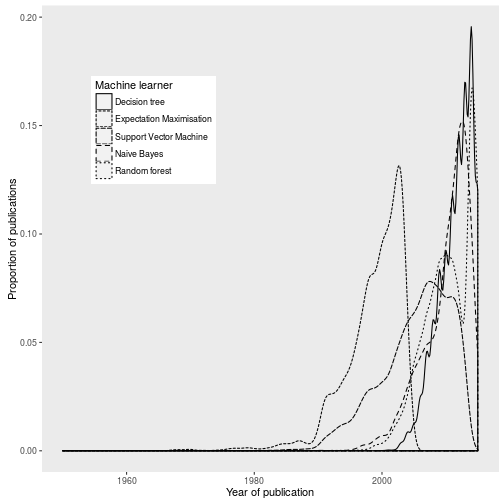
\includegraphics[width=0.9\textwidth]{figure/machine_learning_over_time-1.pdf}
    \caption[Machine learners in scientific literature]{Machine learners in scientific literature. The lines in the graph suggest something of the changing fortunes of machine learners over time. The publication data comes from Thomson Reuter's \textit{Web of Science}. Separate searches were run for each machine learner. In these plots, as in the GoogleTrends data, the actual counts of publications have been normalised. In contrast to the GoogleTrend plots, these plots do not show the relative counts of the publications, only their distribution in time. }
  \label{fig:scientific_lit}
\end{figure}

Similarly, if we attend to the flow of machine learning practices,
devices and techniques in scientific fields, a diversification rather
than a simple scaling-up to industrial-strength infrastructures begins
to appear. Figure \ref{fig:scientific_lit} derives from counts of
scientific publications that mention particular machine learners such as
\texttt{decision\ tree} or \texttt{Naive\ Bayes} in their title, their
abstract or keywords. The curves, which are probability density plots,
\index{graphic!probability density plot} suggest a time-varying
distribution of statements and operations for different techniques. This
crude plot outlines the duration and the ebbs and flows of work on
specific techniques, platforms, knowledges and power relations. Like the
Google Trends searches for \texttt{machine\ learning}, the lines shown
in Figure \ref{fig:scientific_lit} have been normalised in order to
adjust for an overall increase in the volume of scientific publications
over the last five decades.\index{scientific publications} Unlike the
Google Trends search patterns, the scientific literature displays
polymorphous temporalities in which different techniques and operations
diverge widely from each other over the last half century. Crucially for
my purposes, machine learning in the sciences constitutes an a-totality,
a heterogeneous volume and de-centred production of statements.
\index{statements} \index{science!production of statements}

\section{The diagram in critical
thought}\label{the-diagram-in-critical-thought}

As an experiment in the practice of critical thought amidst the
accumulations of data, settings and devices, this book attempts to
\gls{diagram} the data practices of machine learning in respect to
knowledge production. Despite their many operational deployments, the
coming together of algorithm, calculation and technique in machine
learning is not fully coherent or complete. In order to qualify or
specify how machine learners exist in their generality, we would need to
specify their operations at a level of abstraction that neither
attributes a mathematical or algorithmic essence to them nor frames them
as means of production of relative surplus value. Finding ways of
accommodating their diversity, loose couplings and mutability would mean
grasping their operational power and their potential to create new forms
of difference.\footnote{Certain strands of social and cultural theory
  have taken a strong interest in algorithmic processes as operational
  forms of power. For instance, the sociologist Scott Lash distinguishes
  the operational rules found in algorithms from the regulative and
  constitutive rules studied by many social scientists:

  \begin{quote}
  in a society of pervasive media and ubiquitous coding, at stake is a
  third type of rule, algorithmic, generative rules. `Generative' rules
  are, as it were, virtuals that generate a whole variety of actuals.
  They are compressed and hidden and we do not encounter them in the way
  that we encounter constitutive and regulative rules. Yet this third
  type of generative rules is more and more pervasive in our social and
  cultural life of the post-hegemonic order. They do not merely open up
  opportunity for invention, however. They are also pathways through
  which capitalist power works, in, for example, biotechnology companies
  and software giants more generally \autocite[71]{Lash_2007a}.
  \index{Lash, Scott!on generative rules}
  \index{power!operational distinguished from regulatory}
  \end{quote}

  The term `generative' is somewhat resonant in the field of machine
  learning as generative models, models that treat modelling as a
  problem of specifying the operations or dynamics that could have given
  rise to the observed data, are extremely important.
  \index{machine learner!generative}}

Diagrams -- a form of drawing that smooths away many frictions and
variations -- \index{diagram!abstraction as} practically abstract.
(Gilles Deleuze, in his account of Michel Foucault's philosophy presents
diagrams as centres of power-knowledge: `What is a diagram? It is a
display of the relations between forces which constitute power in the
above conditions \ldots{} the diagram or abstract machine is the map of
relations between forces, a map of destiny, or intensity'
\autocite[36]{Deleuze_1988}\index{Deleuze, Gilles!on diagrams}).
Diagrams retain a connection to forms of doing, such as `learning from
experience,' that idea-centric accounts of abstraction sometimes
struggle with. Perceptually and operationally, they span and indeed
criss-cross between human and machine machine learners. As we will see,
they form an axis of human-machine relations in machine learning, and a
significant site of invention and emergence. They accommodate
compositional substitutions, variations and superimpositions, as well as
a play or movement amongst their often heterogeneous elements.
Occasionally, perhaps rarely (Foucault as we will see characterises
statements by their rarity amidst
accumulation\index{statements!rarity of}), by virtue of its composition,
diagrams bring something new into the world.

Both the commonality and specificity (indeed the specific commonality)
of machine learners would be hard to grasp without being able to trace
their diagrammatic composition. Similarly, in order to understand the
operational formation \index{operational formation} associated with
machine learning, the connections between data structures,
infrastructures, processors, databases and lives need to be mapped. One
path to follow in doing this - certainly not the one for everyone -- is
to inhabit and recognise oneself as a machine learner by occupying
associated subject positions (the programmer or software developer, the
statistics or computer science student, the modeller, the researcher,
the data scientist, etc.) In moving between some of these subject
positions, the densely operational indexes of mathematical formalisms
begin to unravel.

Diagrams can be drawn in multiple ways, using various materials and
inscriptive practices. Perhaps naively interpellated by the claim of
machine learning to know differently, I use code and software
implementations, graphical plots and mathematical expressions absorbed
or copied from textbooks, blogs, online videos and the heavy
accumulation of scientific publications from many disciplines (for
instance, as seen in figure \ref{fig:scientific_lit}), together with the
theoretical resources of a media-focused \gls{archaeology} of knowledge
and a science studies-informed ethnographic sensibility towards always
situated and configured infrastructural and calculative practices.

From my own learning to machine learn,
\index{learning!to do machine learning} I draw six major machine
learning operations diagrammatically: vectorisation, optimisation,
probabilisation, pattern recognition, regularization and propagation.
These generic operations intersect in a diagram of machine learning
spanning hardware and software architectures, organizations of data and
datasets, practices of designing and testing models, intersections
between scientific and engineering disciplines, and professional and
popular pedagogies. With varying degrees of formalization and
consistency, these operations might also occasion or provoke some
creative, resistive or re-distributive moves for critical thought in
relation to differences, materiality, experience, agency or power.
\index{diagram!of operations} They are the topics of chapters
\ref{ch:vector}-\ref{ch:subject}. A summary of the operations can also
be found near the beginning of the concluding chapter.

My somewhat risky a-critical immersion in technical practice seeks to
support an alternative account of machine learning, an account in which
some feeling of agency movement can take root. Mundane technical
practices, sometimes at a quite low level (for instance, vectorisation)
and other times at a high level of formalization (for instance, in
discussing mathematical functions) are elements to be drawn -- sometimes
literally, sometimes operationally -- on a diagram. The
\gls{archaeology} of the operational formation of machine learning does
not unearth the footprint of a strategic monolith, but highlights the
local relations of force that feed into the generalization and plurality
of the field in both its monumental accumulations and peripheral
variations.
